\subsection{Modello di programmazione}
ARM v-7 è un'architettura RISC a 32 bit, in cui la maggior parte delle istruzioni esegue in un solo colpo di clock. L'insieme di registri è \textbf{Ortogonale} (quando si afferma che l'insieme dei registri di un processore è ortogonale, si intende che tutti i registri possono essere utilizzati in modo intercambiabile all'interno delle istruzioni della CPU. In altre parole, ogni istruzione che opera sui registri può essere applicata a qualsiasi registro, senza restrizioni o privilegi particolari per alcuni di essi). Inoltre è un architettura \textit{load-store}, ovvero si può accedere alla memoria principale solo attraverso le due istruzioni load e store, mentre tutte le altre istruzioni operano su registri interni del processore (scelta tipica delle architetture RISC). 
Molte architetture ARM supportano due famiglie di istruzioni:
\begin{itemize}
    \item ARM Native - set di istruzioni a 32 bit;
    \item Thumb - set di istruzioni a 16/32 bit, meno efficienti ma in generale più compatte, ideali per sistemi in cui è fondamentale il management della memoria. 
\end{itemize}

ARM ha sette diverse modalità operative, ognuna ha uno stack dedicato ed usa un determinato sottoinsieme di regsitri. Questa scelta è denominata \textbf{Register bamking}: Il register banking nei processori ARM è una tecnica che consiste nell’avere più copie fisiche (banchi) di alcuni registri, usate in base alla modalità di esecuzione o al tipo di eccezione. Questo consente di velocizzare i context switch (cambi di contesto), evitando il salvataggio immediato dei registri in memoria. Lo scopo è quello di ottimizzare il cambio di contesto, evitando di salvare e ripristinare lo stato precedente, passando istantaneamente a un set alternativo di registri già pronti (figura \ref{img:register_banking}).

\begin{figure}[h!]
    \centering
    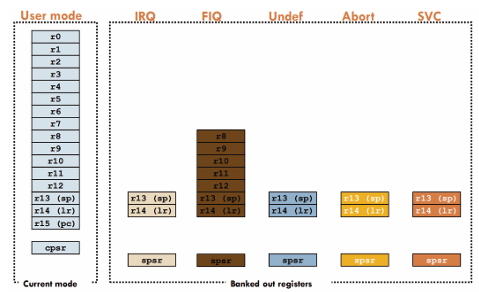
\includegraphics[width=.7\textwidth]{img/register_banking.png}
    \caption{Sistema Register Banking}
    \label{img:register_banking}

\end{figure}

Le modalità operative sono:
\begin{itemize}
    \item \textbf{SVC}: Stato di avvio, il processore può raggiungere questo stato eseguendo una SuperVisor-Call;
    \item \textbf{FIQ}: Stato raggiunto quando la linea Fast Interrupt ReQuest rileva un segnale;
    \item \textbf{IRQ}: Stato raggiunto quando la linea Interrupt ReQuest rileva un segnale;
    \item \textbf{Abort}: Stato raggiunto quando viene effettuato un accesso illegale in memoria;
    \item \textbf{Undef}: Stato raggiunto quando viene tentata un'istruzione non esistente o non definita in memoria;
    \item \textbf{System}: modalità sistema, permette di accedere ai registri \textit{user} in maniera privilegiata;
    \item \textbf{User}: modalità utente, unica modalità non privilegiata, destinata ai programmi utente.
\end{itemize}

SVC, FIQ, IRQ, Abort e Undef sono anche definite modalità 'eccezione'.

Su ARMv7-M le modalità operative invece sono solo due:
\begin{itemize}
    \item \textit{Thread Mode}: modalità per programmi utente. \uppercase{è} la modalità in cui si avvia il processore;
    \item \textit{Handle Mode}: usata da tutti i gestori delle eccezioni e delle itnerruzioni.
\end{itemize}

In questo processore privilegi, stack e registri possono essere configurati.

\subsection{Gestione delle Eccezioni}
Definiamo \textit{eccezione} in questo contesto qualsiasi evento che interrompa il normale flusso di esecuzione di un programma. Queste possono essere interne (memory faults) o esterne (bus error), possono essere inoltre sincrone (esecuzione di una SVC, ovvero una supervisor call) o asincrone (richiesta di una periferica). 

Dal punto di vista architetturale, le interrupt sono vettorizzate. Questo presuoppone che esista una \textit{interrupt vector table} e che esista un intermediario (qualcosa di simile al PIC \ref{par:PIC}) tra processore e sorgenti di interruzione, che può essere un \textbf{Generic Interrupt Controller} nei sistemi A e R, mentre un \textbf{Nester Vector Interrupt Controller} nei sistemi M. 

Le funzioni principali del GIC sono:
\begin{itemize}
    \item Ricevere interruzioni hardware da periferiche;
    \item Classificare le itnerruzioni in base a priorità, tipo  e target;
    \item Decidere a quale \textit{core} inoltrare l'interruzione;
    \item Mascherare, abilitare, cancellare interrupt.
\end{itemize}

NVIC è un oggetto simile ma progettato per il real time, con latenza minima e gestione semplice delle interruzioni nidificate. \uppercase{è} di solito integrato nel core. 

\begin{figure}[ht]
    \centering
    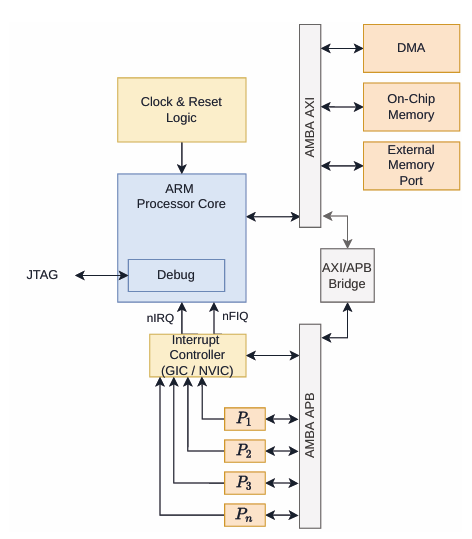
\includegraphics[width=.5\textwidth]{img/arm_eccezioni_arch.png}
    \caption{Vista architetturale}
    \label{img:arm_eccezioni}
\end{figure}

Quando viene scatenata un'eccezione, viene gestita nel seguente modo:
\begin{itemize}
    \item 1 - Il processore salva il PC nel registro \textbf{LR\_<modalità>};
    \item 2 - Il processore salva il CPSR (stato corrente del processore) in \\ \textbf{SPSR\_<modalità>};
    \item 3 - Cambia la modalità operativa (IRQ mode o FIQ mode);
    \item 4 - Disabilita se necessario altre eccezioni;
    \item 5 - Consulta il vettore delle interruzioni;
    \item 6 - Esegue il codice dell'handler;
    \item 7 - Ripristino di CPSR e valore del PC.
\end{itemize}

Il salvataggio di CPSR non è altro che un salvataggio dei registri correntemente usati.

\subsection{Differenze principali tra architetture}
Illustriamo le principali differenza tra ARM, MIPS e M68K:

\begin{itemize}
    \item Instruction Set Architecture (ISA):
    \begin{itemize}
        \item M68k dispone di molte istruzioni in grado di accedere alla memoria principale \textit{direttamente};
        \item MIPS e ARM hanno un'ISA di tipo \textit{load-store}: solo queste possono accedere alla memoria principale, le altre operazioni sono eseguite sui registri interni;
    \end{itemize}
    \item lunghezza istruzioni:
    \begin{itemize}
        \item M68k dispone di istruzioni a lunghezza variabile;
        \item MIPS e ARM dispongono solo di istruzioni a lunghezza fissa;
    \end{itemize}
    \item Modi di indirizzamento:
    \begin{itemize}
        \item M68k dispone di 6 modi di indirizzamento, più le varianti per un totale di 14;
        \item MIPS ne ha soltanto 3;
        \item ARM ha gli stessi di MIPS più \textbf{pc-relative} utilizzabile nella load per caricare costanti salvate in area programma, \textbf{pre-indexed} e \textbf{post-indexed} utilizzabili per incrementare automaticamente il registro prima o dopo l'accesso in memoria;
    \end{itemize}
    \item Flusso di controllo:
    \begin{itemize}
        \item in MIPS le istruzioni testano il contenuto di un registro;
        \item in ARM/68k le istruzioni testano lo stato del processore (le istruzioni aritmetiche e logiche alterano lo stato);
    \end{itemize}
    \item Subroutines:
    \begin{itemize}
        \item MIPS/ARM salvano l'indirizzo di ritorno in un registro;
        \item M68k salva l'indirizzo di ritorno sullo stack; 
    \end{itemize}
\end{itemize}

